
\section{Perceived versus ``true'' risk}

With the true risk proxy from the real-time machine-learning forecasting, denoted as $\widehat{JF}^*$ and $\widehat{JS}^*$, respectively, we can directly estimate the degree of belief distortion, namely the extent to which perceived job risks $\widetilde{JF}$ and $\widetilde{JS}$ deviate from rational ex-ante job risks. In particular, we regress $\widetilde{JF}$ and $\widetilde{JS}$ on the machine-efficient risk forecasts, $\widehat{JF}^*$ and $\widehat{JS}^*$, respectively. We use the log values in both sides of the equation so that the coefficient can be interpreted as the elasticity of beliefs with respect to changes in real-time risk. A coefficient of unity corresponds to the situation where perceived job risks fully react to real-time rational risk, e.g. no under/overreactions.

For each one percentage point increase in real-time job-finding forecast, the average perceived job-finding rate increases by 0.5 percentage points. This suggests that perceived job finding follows real-time job finding rate forecasts relatively well. But a coefficient of only half is still indicative of underreaction in job finding expectations. Figure \ref{fig:survey_versus_machine} plots the perceived risk, real-time machine-efficient risk forecasts, and ex-post transition rates. 

\begin{equation}
\label{eq:jf_est}
   \log(\widetilde{{JF}}_{t+3|t}) = 1.92 + \textbf{0.51} \log(\widehat {JF}^*_{t+3|t}) + \epsilon_{t}
\end{equation}


\begin{figure}[pt] 
\centering 
	\caption{Survey perceived job risks versus machine-efficient risk forecasts (0-1)} 
	\label{fig:survey_versus_machine}
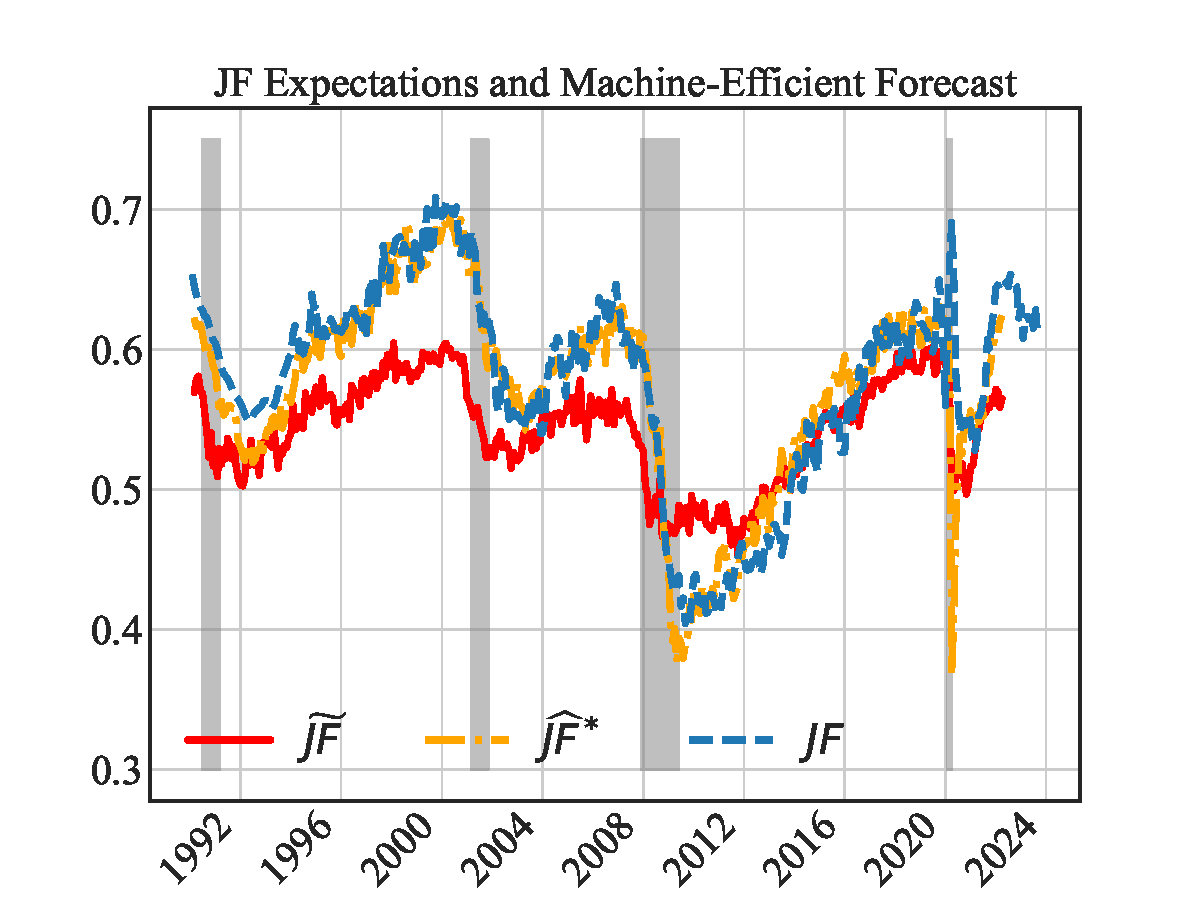
\includegraphics[width=0.7\linewidth]{text/chapter2/Figures/real_time_survey_machine_realization_1step_JF.pdf} \\
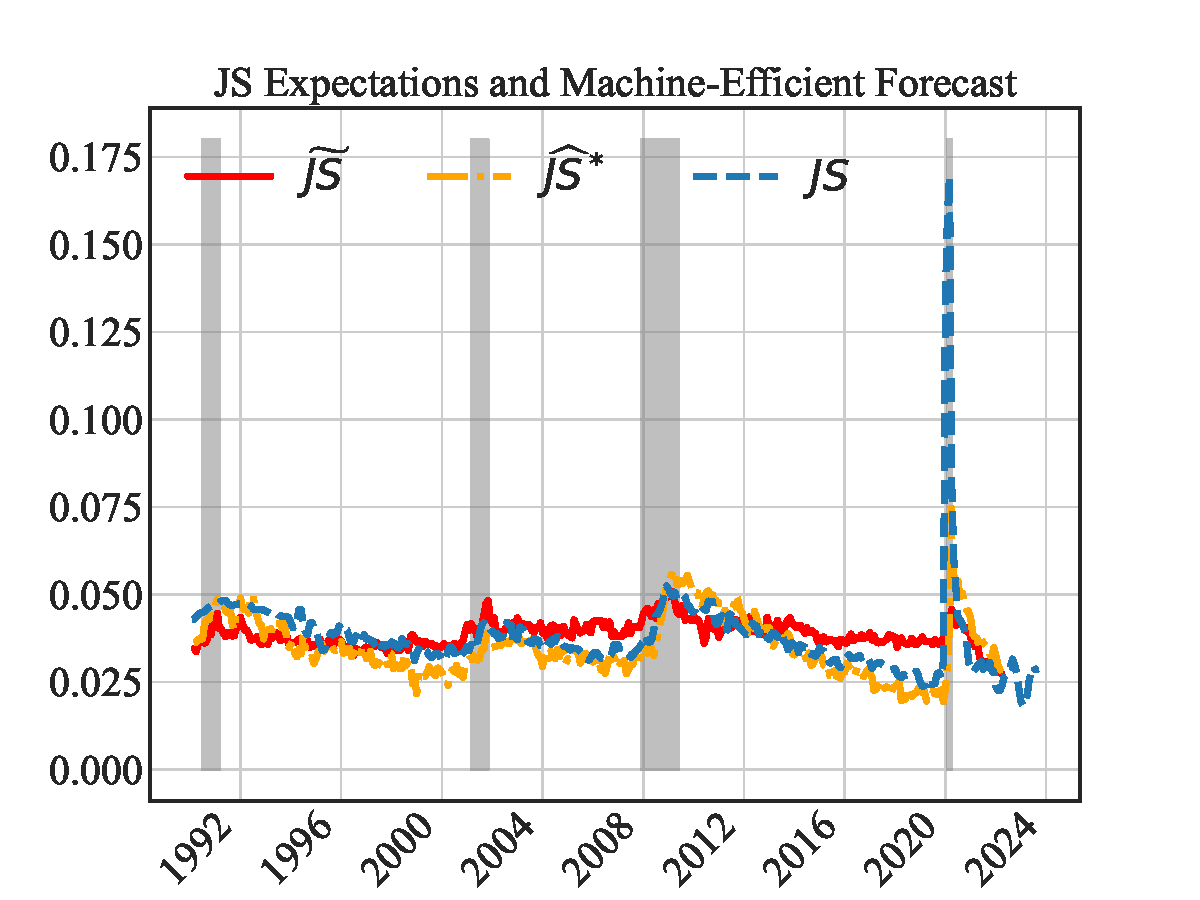
\includegraphics[width=0.7\linewidth]{text/chapter2/Figures/real_time_survey_machine_realization_1step_JS.pdf} 
  \floatfoot{\footnotesize{the charts plot (in the scale of 0-1) perceived job risk, real-time machine-efficient forecast, and realized job flow rates.}}
\end{figure}

Perceived job-separation probabilities are less correlated with the real-time risk, with a regression coefficient $\widehat{JS}^*_{t+3|t}$ being $0.31$, implying a one-third percentage point increase in response to each one percentage point increase in machine forecasts. Perceived job separation fails to incorporate about 80\% of the predictable job separation transitions. 

In addition, similar to perceived job finding, the constant term of the regression is positive, implying on average an upward bias in the perceived job separation rate.

\begin{equation}
\label{eq:js_est}
 \log(\widetilde {{JS}}_{t+3|t}) = 1.13 + \textbf{0.19} \log(\widehat {JS}^*_{t+3|t}) + \epsilon_{t}
\end{equation}


\subsection{Information rigidity in job beliefs}

The tests presented in the previous section using forecast errors reject the null of FIRE and imply information rigidity, but it does not give us an exact degree of information rigidity that can be used to generate quantitative model implications. To do so, we follow a large body of literature to specify a widely used model of expectation formation capturing information rigidity: Sticky Expectations (SE).\footnote{\cite{mankiw2002sticky}, \cite{carroll2003macroeconomic}, and  \cite{coibion2015information}.}

Sticky Expectation posits a very tractable mechanism of underreaction mechanism of beliefs in the population average. In particular, in each period, each agent learns about the most up-to-date information regarding the aggregate economy (the true underlying real-time job-finding probability) at a constant and time-independent rate of $\lambda$. Therefore, the average belief under SE mechanism follows a recursive formula as below. 

\begin{equation}
\label{equation:se}
\widetilde {JF}_{t+3|t} = (1-\lambda) \widetilde {JF}_{t+3|t-1} + \lambda {JF}^*_{t+3|t} 
\end{equation}

The intuition behind this equation is that the average expectation depends on both the average expectation of the $(1-\lambda)$ fraction of agents who did not update at time $t$ and the FIRE expectation of the $\lambda$ fraction of updated agents. In the special case of full-updating, $\lambda = 1$, the above equation collapses into the FIRE case.\footnote{A number of studies have estimated the updating rate $\lambda$ to be significantly lower than one, based on survey expectations of inflation, unemployment and other macroeconomic variables, e.g. \citet{mankiw2002sticky}, \citet{carroll2003macroeconomic}, \cite{coibion2012can}, etc. In the literature, such information rigidity can be also microfounded by another class of models, namely the noisy information, where agents learn about the true state of the world via noisy public and private signals. Like SE, it generates a serial correlation of forecast errors as shown at the beginning of the paper, but it does not exactly have a prediction as in Equation \ref{equation:se}. }

Our estimated Equation \ref{eq:jf_est} and Equation \ref{eq:js_est} can be almost squarely interpreted within the SE framework. In particular, the updating rate of job-finding expectations is about $\widehat\lambda^{JF} = 0.51$ and $\widehat\lambda^{JS} = 0.19$ for job separations. Both are significantly different from unity, rejecting the null hypothesis of perfect updating. 

When the lagged perceived job risks are controlled in the same regression, the coefficient remains in a similar range. In addition to the true real-time risks, we also control past information such as the realized job finding and separation flow rates or aggregate economic variables. The estimated rigidity does not vary much.

Although the information rigidity as formulated by SE model fits the correlation between perceived job risks and true real-time risks well, there remains the big gap between the SE-model-implied time series of perceived job risks $\widetilde{JF}^{SE}$versus the observed perceived job risks $\widetilde{JF}$ as plotted in Figure \ref{fig:fitted_se} where we plug in the estimated $\hat \lambda^{JF}$ and $\hat \lambda^{JS}$ into the Equation \ref{equation:se}. The perceived job risk sequences more or less center around the true real-time risks, with mild deviations. It shows less time-variations, which does capture the underreaction of perceptions to real-time conditions. 



\begin{comment}
Assuming the true underlying process of job finding rate is an AR(1) process with a degree of persistence of $\rho$. 

\begin{equation}
    JF_{t,t+3} = \rho \text{JF}_{t-1,t+2} + \omega_{t+3}
\end{equation}

Then Equation \ref{equation:se} can be further rewritten as the following. 


\begin{equation}
\label{equation:se2}
\widetilde {JF}_{t+3|t} =  (1-\lambda) \rho\widetilde {JF}_{t+3-1|t-1} + \lambda \rho^h {JF}_{t-h,t}
\end{equation}

With an estimated AR(1) coefficient $\rho=0.99$ using the realized monthly job finding rate in the first step, and taking the real-time job-finding rate as given, we can then estimate\footnote{In practice, we also estimate the initial value of the belief $\tilde {JF}_{3|0}$.}
 the value of the monthly $\lambda$ to match the SE-model implied monthly job finding expectations and the observed/imputed job finding expectations. The baseline estimation suggests a monthly value of $\lambda = 0.30$, which implies only one-third of the population updates each month about the aggregate job finding rate. Although our added SE mechanism does not fully capture the fluctuations of the job-finding expectations, it does demonstrate a degree of underreaction that was also seen in the observed/imputed expectation. (See Figure \ref{fig:fitted_se})

\end{comment}

       \begin{figure}[pt]
    	\caption{The Estimated Sticky Expectation Model of Perceived Job Risks (0-1)}
	\label{fig:fitted_se}    
    	\begin{center}
		\adjustimage{max size={0.7\linewidth}}{text/chapter2/Figures/real_time_survey_machine_realization_1step_SE_JF_fit.pdf}  \\
  \adjustimage{max size={0.7\linewidth}}{text/chapter2/Figures/real_time_survey_machine_realization_1step_SE_JS_fit.pdf} 
    	\end{center}
     
    	
    	  \floatfoot{\footnotesize{the figures plot the perceived job risk ($\widetilde{JF}$ and $\widetilde{JS}$) versus their fitted value based on the estimation of Equation \ref{eq:jf_est} and \ref{eq:js_est}, in addition to the realized job transition rates ($JF$ and $JS$.), respectively. All rates are on a scale of 0-1. } }
    \end{figure}
    
\subsection{Heterogeneity in job risks}

Our analysis so far assumes homogeneous job risks, which means that the perceived job risks by different workers are supposed to react to the true aggregate risk by the same degree in the absence of belief distortion. But in reality, job risks are widely heterogeneous across workers \citet{hall2019job,ahn2020heterogeneity,gregory2021alpha}. So are the perceived risks, as shown in \cite{mueller2021job,wang2023perceived}. \cite{guvenen2014nature} shows that heightened income risks during recessions can be in part predicted by observable factors measured prior to recessions. \cite{patterson2023matching} shows that the positive correlation between workers' marginal propensity to consume (MPCs) and the cyclicality of their income amplifies recessions compared to a world with equal income exposure. A similar argument can be made in the space of job risks. We therefore consider it to be important to study ex-ante heterogeneity in job risks. Unlike the common countercyclical risks that drive time-varying fluctuations, the presence of risk heterogeneity causes business cycle fluctuations via its heterogeneous incidences.  

Meanwhile, the fact that workers face different degrees of job risks is naturally another important reason for why average perceptions underreact to the real-time conditions. To see this point clearly, assume an individual worker $i$'s $JF$ has an idiosyncratic loading $\eta_{i,t}$ from the aggregate job finding rate ${JF}_t$. (Equation \ref{eq:hetero_risks}). Where each individual $i$ has their respective expectations of their own heterogeneous risk $\widetilde{JF}_{i,t}$. We further make the assumption that people know perfectly about their heterogeneous factor $\eta_{i,t}$, which makes the last equality hold in the second line of the Equation \ref{eq:hetero_risks}. 

  \begin{equation}
  \label{eq:hetero_risks}
   \begin{split}
   &    \text{JF}_{i,t} = \eta_{i,t}\text{JF}_{t}  \\
&    \widetilde{\text{JF}_{i,t}} = \mathbb{E}_i(\text{JF}_{i,t})=\mathbb{E}_i(\eta_{i,t}\text{JF}_{t}) = \eta_{i,t} \mathbb{E}_i(\text{JF}_{t})
   \end{split}
   \end{equation}


If the following equation holds, namely if average perceived job risks across agents converge to the aggregate job risks $JF_t$ depends on at least two factors. The first is the cross-sectional distribution of $\eta_{i,t}$. The second is the expectation patterns of individuals toward aggregate job risk. Even if all workers correctly perceive ${JF}_t$, which implies $\mathbb{E}_i(\text{JF}_{i,t}) = {JF}_t \forall i$, the heterogeneity in job risks still matter for the behaviors of average perceived job risk.

\begin{equation}
  \widetilde{JF}_t = \frac{\sum     \mathbb{E}_i(\text{JF}_{i,t})}{N}=\frac{\sum \eta_{i,t}}{N}JF_t  \overset{?}{=}  \text{JF}_{t}
\end{equation}

Such an aggregation through the distributional effects of aggregate job risk on individual workers, even in the absence of belief distortion, would also potentially imply a wedge between average perception and true aggregate risk. Imagine the shocks to $JF_t$ are highly persistent while the idiosyncratic loadings $\eta_{i,t}$ are entirely transitory and agents perceive these components correctly. That would imply that the average perceived risks $\widetilde{JF}_t$ are less responsive to aggregate risks $JF_t$ by a degree less than unity. 

The importance of heterogeneity in job risks in understanding perceived job risks is emphasized by \cite{mueller2021job}.  They show that both ex-ante heterogeneity and underreaction to variations in job-finding rate \textit{across workers} and \textit{over unemployment spells} are important to explain the patterns of job-finding perceptions. To the extent that such beliefs induce self-insurance behaviors through job search, underreaction to the heterogeneity and duration-dependent variations results in a larger dispersion in job-finding outcomes. What this paper has shown so far is essentially that such underreaction to variations in job risks also exists along the variations of job risks over business cycles at the aggregate level. 

To formally shed light on the role of heterogeneity, we estimate the belief-distortion regression for different percentiles of the perceived job risks. The key assumption is that at any point in the business cycle, workers face different degrees of job risks and are affected by the same aggregate conditions unevenly. 

In particular, instead of the mean perceived job risks in the survey as in Equation \ref{eq:jf_est}, we regress the q-th percentile perceived job risks $\widetilde {JF}^{q}$ and $\widetilde {JS}^q$ $\forall q=\{25,50,75\}$ (Equation \ref{eq:jf_dist_est}) on the same aggregate common real-time risk measure. By doing so, we are asking a very intuitive question: whose expectations are the most reactive to the change in real-time risks? 

   
    \begin{equation}
    \label{eq:jf_dist_est}
    \begin{split}
   \log(\widetilde {JF}^{0.25}_{t+3|t}) = -1.55 + \textbf{1.22} \log(\widehat {JF}^*_{t+3|t}) + \epsilon_{t}  \\
   \log(\widetilde {JF}^{0.5}_{t+3|t}) = 1.54+ \textbf{0.63} \log(\widehat {JF}^*_{t+3|t}) + \epsilon_{t} \\
   \log(\widetilde {JF}^{0.75}_{t+3|t}) = 3.62 + \textbf{0.20} \log(\widehat {JF}^*_{t+3|t}) + \epsilon_{t} 
    \end{split}
\end{equation}

The job-finding perceptions of the 25 percentile worker in terms of their perceptions react to the real-time job-finding rate by a much larger degree than the rest, as implied by the coefficient estimates of 1.22 for this group, as opposed to a 0.63 for the median worker and 0.20 for the worker at the 75 percentile. To put it bluntly, those who usually believe that they cannot easily find a job are the marginal workers whose belief reacts to the real-time job-finding rate the most. A higher-than-one elasticity of beliefs suggests that the beliefs are overreactive to the market finding conditions. 

 \begin{equation}
    \begin{split}
    \log(\widetilde {JS}^{0.25}_{t+3|t})= -0.42 + \textbf{0.46} \log(\widehat {JS}^*_{t+3|t}) + \epsilon_{t}  \\
       \log(\widetilde {JS}^{0.5}_{t+3|t}) = 1.06 + \textbf{0.68} \log(\widehat {JS}^*_{t+3|t}) + \epsilon_{t}  \\
    \log(\widetilde {JS}^{0.75}_{t+3|t}) = 2.57 + \textbf{0.27} \log(\widehat {JS}^*_{t+3|t}) + \epsilon_{t} 
    \end{split}
\end{equation}

In terms of job separation, it is the median-risk workers that have the most sensitive reactions to aggregate real-time job separation rate. The estimates of responses range from 0.46 for 25 percentile workers (almost non-reaction) to 0.68 and 0.27 for the median and 75 percentile workers, respectively.

Taken all together, these estimates suggest conditional on individual heterogeneity in risk exposures, the information rigidity is not as severe as the average perceived job risks. Both overreaction and underreaction in perceptions exist, depending on where the worker is located in the distribution of heterogeneous job risks.

The heterogeneous sensitivities of perceptions with respect to common aggregate risk are probably sensible. In particular, the perceptions of those who perceive high job risks (high separation and low finding risk perceptions) show the highest sensitivity. Business cycles are not just characterized by the change in aggregate job risks, it is probably more accurately seen as a shift in the location of the marginal workers who face the job risks. For instance, in recessions, the marginal worker who faces job loss risk shifts downward from the top 10 percentile of perceived job risk to the 50th percentile. The sensitivity in perceptions helps reveal who is the marginal worker. 

The idea that distributional expectations contain information about the aggregate economy also echoes a few papers that show distributional expectations of households/firms improve the predictions of subsequent aggregate outcomes. It is not always the average agent, but the \emph{marginal} one, whose expectations matter for the macroeconomic outcomes, because the same aggregate shock has different footprints on heterogeneous agents in the economy. 

\begin{figure}[pt] 
\centering 
	\caption{Survey perceived job risks versus machine-efficient risk forecasts by distribution (0-1)} 
	\label{fig:survey_versus_machine_dist}
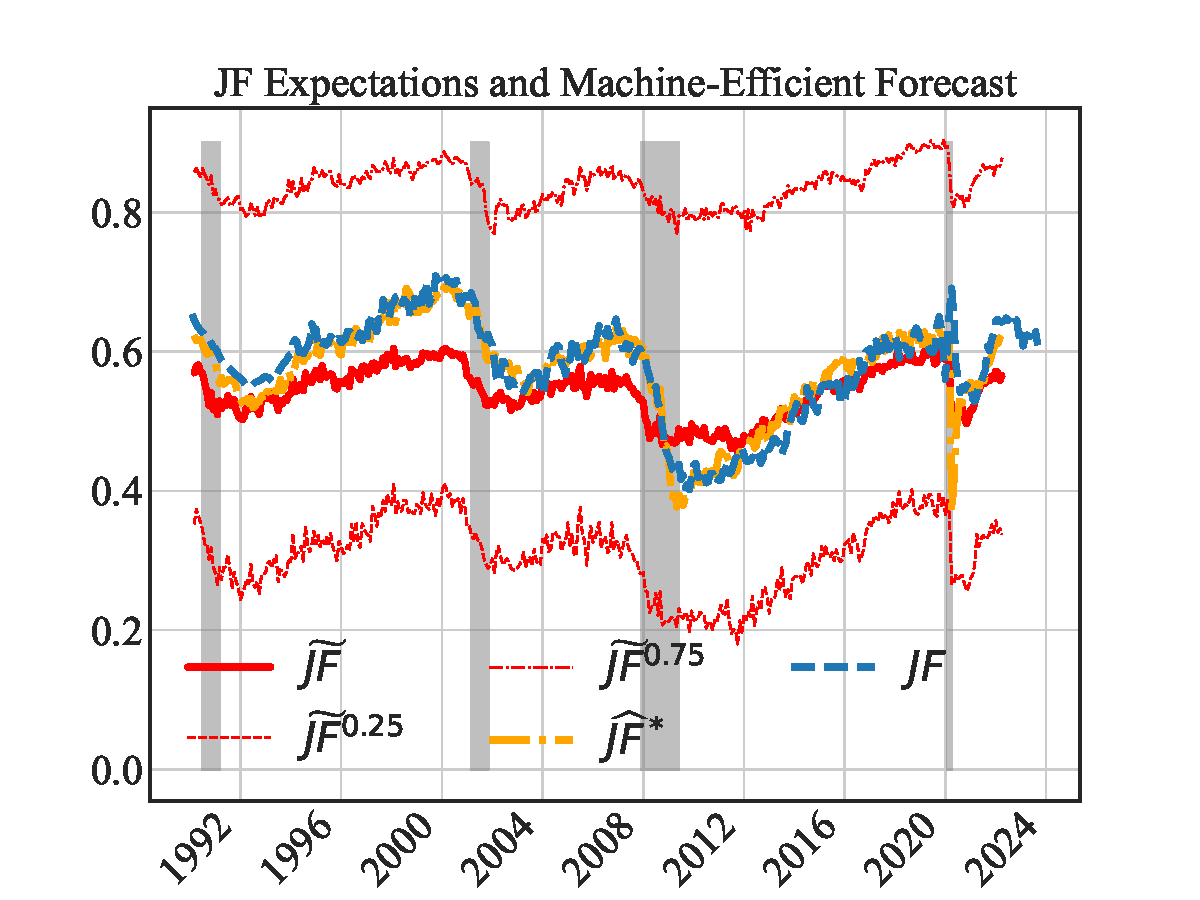
\includegraphics[width=0.7\linewidth]{text/chapter2/Figures/real_time_survey_machine_realization_1step_JF_dist.pdf} \\
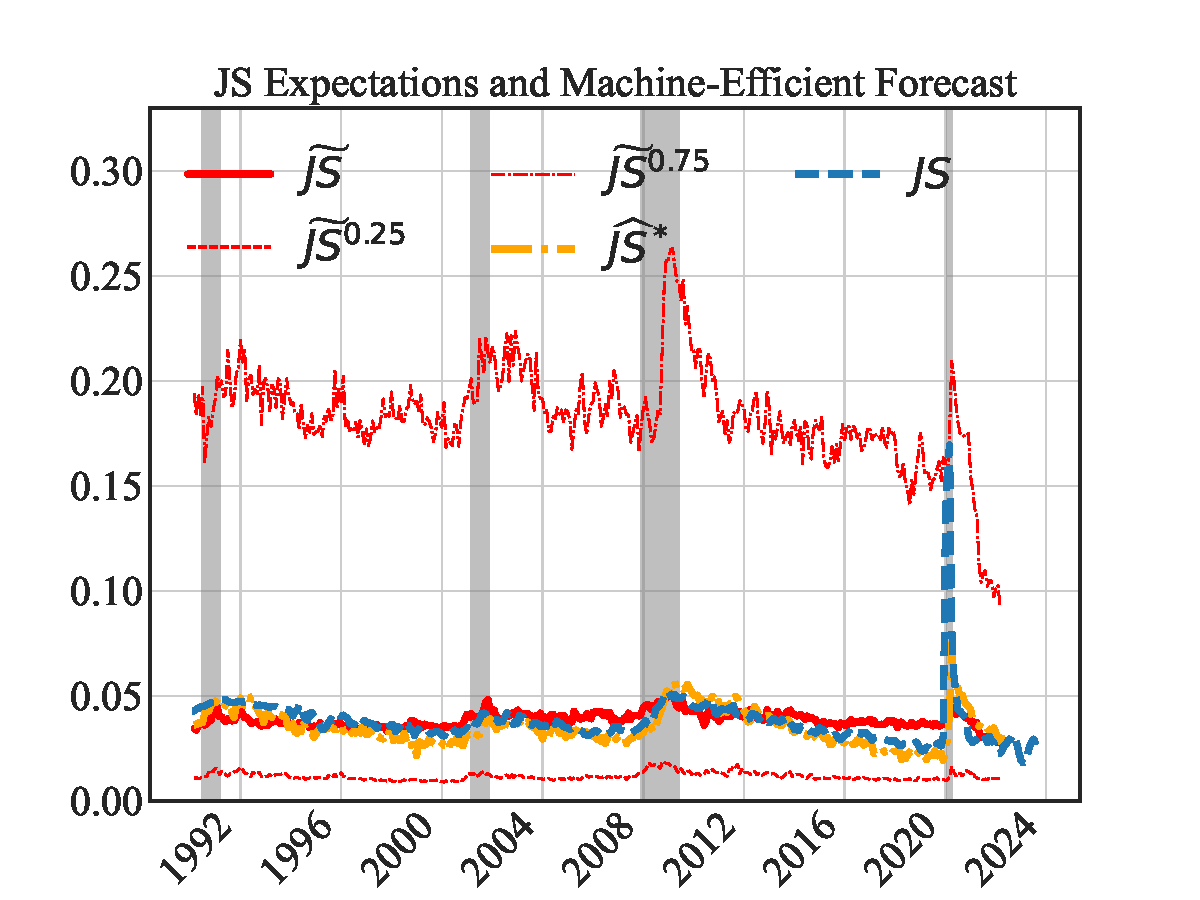
\includegraphics[width=0.7\linewidth]{text/chapter2/Figures/real_time_survey_machine_realization_1step_JS_dist.pdf} 
	\begin{flushleft}\footnotesize {Note: The figures plot the average and heterogeneous perceived job risks at different quantiles, real-time job risks, and realized job transition rates.} \end{flushleft}
\end{figure}


\subsection{Heterogeneous perceptions of job risks}\label{subsec:hetero_beliefs}

Is there heterogeneity in terms of belief distortions in addition to the heterogeneity in true job risks faced by different workers? If the workers who face the most cyclical movements in job risks tend to underperceive such movements -- therefore underinsure -- total consumption fluctuations amplify due to the heterogeneous footprints of uninsured job risks.  

We can shed light on this question along a few observable dimensions, such as education, relying upon the fact that we can create group-specific risk forecasts specifically for each education group, e.g. $\widehat{JF}^{HighEdu*}$,$\widehat{JF}^{MidEdu}$,$\widehat{JF}^{lowEdu*}$, respectively. Using group-specific risk forecasts admits the ex-ante heterogeneous risk exposures of different education groups. 


The estimates are reported below. In terms of job finding, the middle-education group is the most rigid relative to their real-time risk than the low- and high-education workers.  Meanwhile, with job separation, low-education workers underreact to the real-time risks the most, exhibiting the largest degree of information rigidity.  Such patterns are consistent with the patterns in Figure \ref{fig:simple_comparison_by_educ} that different low-education groups underestimate the spike in job separation rate and more strongly react to the decline in job finding at the outbreak of the pandemic than the high-education group. Assuming a strong correlation between education and liquid wealth, \citet{broer2021information} would predict a U-shaped pattern as poor and rich households have the highest incentives to know the current state of the world. Our results support such a claim for job finding, but contradict it for job separation rates. In fact, workers without a high school degree have the weakest reaction in beliefs to changes in realized job separation rates, even though they would have the largest utility penalties of non-optimal precautionary savings.

Despite the differences across workers, however, it is worth emphasizing that overall, all beliefs by all types of groups exhibit rigidity, with the coefficient always below 60 percent. 

  \begin{equation}
    \label{eq:jf_dist_est_edu}
    \begin{split}
      \log(\widetilde {JF}^{LowEdu}_{t+3|t}) = 1.28 + \textbf{0.66} \log(\widehat {JF}^{*LowEdu}_{t+3|t}) + \epsilon_{t}  \\
    \log(\widetilde {JF}^{MidEdu}_{t+3|t}) = 2.53+ \textbf{0.36} \log(\widehat {JF}^{*MidEdu}_{t+3|t}) + \epsilon_{t} \\
    \log(\widetilde {JF}^{HighEdu}_{t+3|t}) = 1.87 + \textbf{0.53} \log(\widehat {JF}^{*HighEdu}_{t+3|t}) + \epsilon_{t}  \\
       \log(\widetilde {JS}^{LowEdu}_{t+3|t}) = 1.1 + \textbf{0.17} \log(\widehat {JS}^{*LowEdu}_{t+3|t})+ \epsilon_{t}  \\
     \log(\widetilde {JS}^{MidEdu}_{t+3|t}) = 0.95+ \textbf{0.35} \log(\widehat {JS}^{*MidEdu}_{t+3|t}) + \epsilon_{t} \\
    \log(\widetilde {JS}^{HighEdu}_{t+3|t}) = 1.08 + \textbf{0.33} \log(\widehat {JS}^{*HighEdu}_{t+3|t}) + \epsilon_{t} 
    \end{split}
\end{equation}
